\documentclass[a4paper,11pt]{extarticle} % тип документа
\usepackage[left=1.6cm,right=1.6cm]{geometry}
%%%Библиотеки
    %\usepackage[warn]{mathtext}	
    \usepackage[T2A]{fontenc}   %Кодировка
\usepackage[utf8]{inputenc} %Кодировка исходного текста
    \usepackage[english, russian]{babel} %Локализация и переносы
    \usepackage{caption}
    \usepackage{listings}
    \usepackage{amsmath, amsfonts, amssymb, amsthm, mathtools}
    \usepackage[warn]{mathtext}
    \usepackage[mathscr]{eucal}
    \usepackage{wasysym}
    \usepackage{graphicx} %Вставка картинок правильная
    \usepackage{indentfirst}
    \usepackage{float}    %Плавающие картинки
    \usepackage{wrapfig}  %Обтекание фигур (таблиц, картинок и прочего)
    \usepackage{fancyhdr} %Загрузим пакет
    \usepackage{lscape}
    \usepackage{xcolor}
    \usepackage[normalem]{ulem}
    
    \usepackage{titlesec}
    \titlelabel{\thetitle.\quad}


%%%Конец библиотек


%Заголовок
\title{Отчет о выполнении лабораторной работы 3.5.1 \\ 
\textbf{Изучение плазмы газового разряда в неоне.}}
\author{Севастьян Черняков и Георгий Чирков}
\date{ ФУПМ МФТИ, 10.10.2023 \\}
\begin{document}
\maketitle 

\textbf{Цель работы}: изучение вольт-амперной характеристики тлеющего разряда, изучение свойств плазмы методом зондовых характеристик.


\textbf{В работе используются}: стеклянная газоразрядная трубка, наполненная изотопом неона, высоковольтный источник питания (ВИП), источник питания постоянного тока, делитель напряжения, резистор, потенциометр, амперметры, вольтметры, переключатели.
\section*{Теория}
\subsection*{Плазма}
В ионизированном газе поле ионов <<экранируется>> электронами. Для поля $\mathbf{E}$ и плотности $\rho$ электрического заряда
$$
\text{div}~\mathbf{E} = 4 \pi \rho,
$$
а с учётом сферической симметрии и $\mathbf{E} = -\text{grad}~\varphi$:
\begin{equation}
\dfrac{d^2 \varphi}{dr^2}+\dfrac{2}{r}\dfrac{d\varphi}{dr}=-4\pi \rho.
\end{equation}
Плотности заряда электронов и ионов (которые мы считаем бесконечно тяжёлыми и поэтому неподвижными)
\begin{equation}
\begin{array}{c}
\rho_e = -ne \cdot \exp\left(\dfrac{e\varphi}{kT_e}\right),\\
\rho_i = ne.
\end{array}
\end{equation}
Тогда из $(1)$ в предположении $\dfrac{e\varphi}{kT_e} \ll 1$ получим
\begin{equation}
\varphi = \dfrac{Ze}{r}e^{-r/r_D},
\end{equation}
где $r_D = \sqrt{\dfrac{kT_e}{4\pi n e^2}}$ -- \textit{радиус Дебая}. Среднее число ионов в сфере такого радиуса 
% \begin{wrapfigure}{r}{4cm}
% 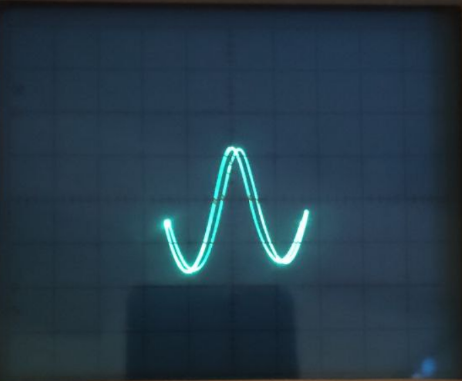
\includegraphics[scale=0.5]{2.png}
% \end{wrapfigure}  
\begin{equation}
N_D = n\dfrac{4}{3}\pi r_D^2.
\end{equation}
Теперь выделим параллелепипед с плотностью $n$ электронов, сместим их на $x$. Возникнут поверхностные заряды $\sigma = nex$, поле от которых будет придавать электронам ускорение:
$$
\dfrac{d^2x}{dt^2}=-\dfrac{eE}{m}=-\dfrac{4\pi n e^2}{m}x.
$$ 
Отсюда получаем \textit{плазменную (ленгмюровскую) частоту} колебаний электронов:
\begin{equation}
\omega_p = \sqrt{\dfrac{4\pi ne^2}{m}}.
\end{equation}
\subsection*{Одиночный зонд}
При внесении в плазму уединённого проводника -- \textit{зонда} -- с потенциалом, изначально равным потенциалу точки плазмы, в которую его помещают, на него поступают токи электроннов и ионов:
\begin{equation}
\begin{array}{c}
I_{e0} = \dfrac{n \langle v_e \rangle}{4}eS,\\
I_{i0} = \dfrac{n \langle v_i \rangle}{4}eS,
\end{array}
\end{equation}
где $\langle v_e \rangle$ и $\langle v_i \rangle$ -- средние скорости электронов и ионов, $S$ -- площадь зонда, $n$ -- плотность электронов и ионов. Скорости электронов много больше скорости ионов, поэтому $I_{i0} \ll I_{e0}$. Зонд будет заряжаться до некоторого равновестного напряжения $-U_f$ -- \textit{плавающего потенциала}.\\
% \begin{wrapfigure}{r}{5.5cm}
% 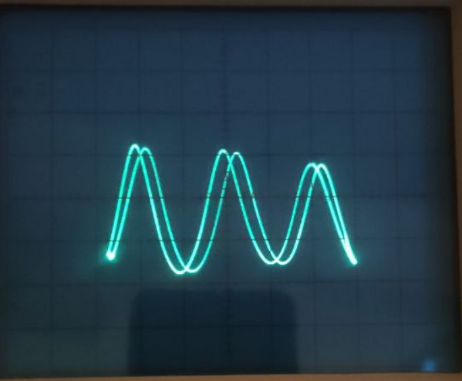
\includegraphics[scale=0.5]{3.png}
% \end{wrapfigure}  
В равновесии ионный ток мало меняется, а электронный имеет вид
$$
I_e = I_0 \exp\left( -\dfrac{eU_f}{kT_e} \right).
$$
Будем подавать потенциал $U_\text{з}$ на зонд и снимать значение зондового тока $I_\text{з}$. Максимальное значение тока $I_{e\text{н}}$ -- электронный ток насыщения, а минимальное $I_{i\text{н}}$ -- ионный ток насыщения. Значение из эмпирической формулы Бомона:
\begin{equation}
I_{i\text{н}} = 0.4 neS \sqrt{\dfrac{2kT_e}{m_i}}.
\end{equation}
\subsection*{Двойной зонд}
Двойной зонд -- система из двух одинаковых зондов, расположенных на небольшом расстоянии друг от друга, между которыми создаётся разность потенциалов, меньшая $U_f$. Рассчитаем ток между ними вблизи $I=0$. При небольших разностях потенциалов ионные токи на оба зонда близки к току насыщения и компенсируют друг друга, а значит величина результирующего тока полностью связана с разностью электронных токов. Пусть потенциалы на зондах
$$
U_1 = -U_f + \Delta U_1,
$$
$$
U_2 = -U_f + \Delta U_2.
$$
Между зондами $U = U_2 - U_1 = \Delta U_2 - \Delta U_1$.
Через первый электрод
\begin{equation}
I_1 = I_{i\text{н}} + I_{e1} = I_{i\text{н}} - \dfrac{1}{4}neS\langle v_e\rangle \exp\left(-\dfrac{eU_f}{kT_e}\right)\exp\left(\dfrac{e\Delta U_1}{kT_e}\right)=I_{i\text{н}}\left(1 - \exp\left( \dfrac{e\Delta U_1}{kT_e} \right)\right).
\end{equation}
Аналогично через второй получим
\begin{equation}
I_2 = I_{i\text{н}}\left(1 - \exp\left( \dfrac{e\Delta U_2}{kT_e} \right)\right)
\end{equation}
  
Из $(7)$ и $(8)$ с учётом последовательного соединение зондов ($I_1 = -I_2 = I)$:
$$
\Delta U_1= \dfrac{kT_e}{e}\text{ln}\left(1 - \dfrac{I}{I_{i\text{н}}}\right)
$$
$$
\Delta U_2= \dfrac{kT_e}{e}\text{ln}\left(1 + \dfrac{I}{I_{i\text{н}}}\right)
$$

Тогда итоговые формулы для разности потенциалов и тока

\begin{equation}
U = \dfrac{kT_e}{e}\text{ln}\dfrac{1 - I/I_{i\text{н}}}{1 + I/I_{i\text{н}}}, 
I = I_{i\text{н}} \text{th}\dfrac{eU}{2kT_e}.
\end{equation}
Реальная зависимость выглядит несколько иначе и описывается формулой 
% \begin{wrapfigure}{l}{7cm}
% 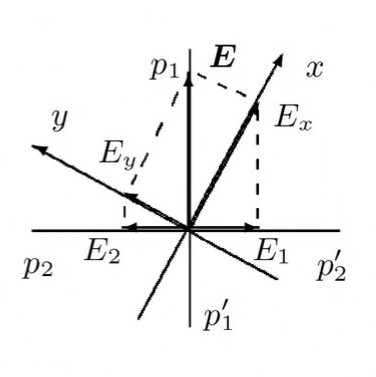
\includegraphics[scale=0.8]{4.png}
% \vspace{+30pt}
% \end{wrapfigure}
\begin{equation}
I = I_{i\text{н}} \text{th}\dfrac{eU}{2kT_e} + AU.
\end{equation}
Из этой формулы можно найти формулу для $T_e$: для $U=0$ мы найдём $I_{i\text{н}}$, продифференцируем в точке $U=0$ и с учётом $\text{th}~\alpha \approx \alpha$ при малых $\alpha$ и $A\rightarrow 0$ получим:
\begin{equation}
kT_e = \dfrac{1}{2}\dfrac{eI_{i\text{н}}}{\dfrac{dI}{dU}|_{U=0}}.
\end{equation}

\section*{Ход работы}
Измеряем напряжение зажигания в лампе: $<U_{\text{заж}>} = 211\pm 1$ В.\\
С помощью вольтметра $V_1$ и амперметра $A_1$ снимаем ВАХ разряда $U_1=f(I_p)$ для тока в диапазоне $0.5 \div 5$ мА (см. Таблица 1).
Построим график:\\
\begin{figure}[h]
\centering
% 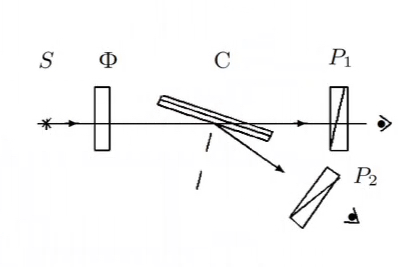
\includegraphics[scale=0.6]{6.png}
\caption{Вольт-амперная характеристика разряда.}
\end{figure}\\
По наклону определим максимальное сопротивление заряда (с учётом того, что вольтметр подключен через делитель напряжения с коэффициентом 10): $R_{max} = (8.5\pm 0.2)\cdot 10^4~\text{Ом}$.\\
С помощью вольтмертра $V_2$ и амперметра $A_2$ снимем ВАХ двойного зонда $I_2 = f(U_2)$ при фиксированного токе разряда $I_p$ в трубке в диапозоне $-25 \div 25$ В, процессе измерений меняя полярность зонда при нулевом токе. Измерения проведём для $I_p = 5$ мА, $I_p = 3$ мА  и $I_p = 1.5$ мА (Таблица 2).\\
Результаты измерений представим на графиках с отцентрованными $\left(I_0 = \dfrac{1}{2}\sum I\right)$:
\newpage
% \begin{figure}[h]
%     \centering
%     \subfloat[ВАХ двойного зонда, $I = 5.0$ мА.]{{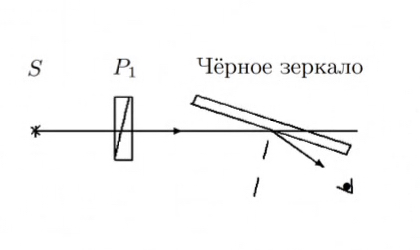
\includegraphics[width=0.5\textwidth]{5.png}}}
%     \subfloat[ВАХ двойного зонда, $I = 3.0$ мА.]{{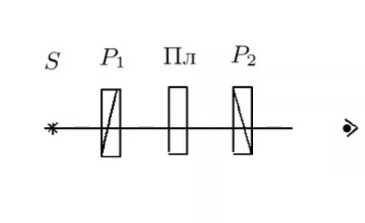
\includegraphics[width=0.5\textwidth]{7.png}}}\\
%     \subfloat[ВАХ двойного зонда, $I = 1.5$ мА.]{{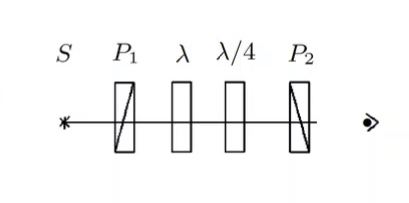
\includegraphics[width=0.5\textwidth]{8.png}}}
% \end{figure}
Приближая кривые формулой $I = A \text{th}(BU) + CU$, найдём токи насыщения $I_{i\text{н}}$ и температуры электронов $T_e$.\\
Считая концентрации ионов и электронов равными, найдём их, пользуясь формулой (7). Рассчитаем плазменную частоты $\omega_p$ по формуле (5) и радиус Дебая $r_D$, оценим среднее число ионов в дебаевской сфера $N_D$ по формуле (4) и  степень ионизации $\alpha$, приняв $P\approx 1$ мбар, и занесём все результаты в таблицу.
\begin{table}[h!]
\centering
\begin{tabular}{|c|c|c|c|c|c|c|}
\hline
$I_p$, мА  & $T_e$, $10^4$ К   & $n_e$, $10^{15}$ м$^{-3}$ & $\omega_p$, $10^4$ рад/c & $r_D$, $10^{-5}$ см & $N_D$ & $\alpha$, $10^{-7}$ \\ \hline
5.0   & $41\pm 4$ & $58\pm 6$     & $144\pm 10$   & $49\pm 3$      & 30 & 24\\ \hline
3.0   & $42\pm 4$ & $33\pm 4$     & $107\pm 9$    & $66\pm 5$      & 40 & 13\\ \hline
1.5   & $41\pm 6$ & $16\pm 2$    & $75\pm 8$     & $94 \pm 10$     & 57 & 7\\ \hline
\end{tabular}
\end{table}
\newpage
\section*{Результаты измерений}
\begin{table}[h]
\centering
\begin{tabular}{|c|c|c|c|c|c|c|c|c|c|c|c|}
\hline
$U_1$, В & 23.9 & 24.15 & 24.35 & 24.4 & 24.81 & 25.40 & 26.20 & 27.71 & 30.92 & 34.19 & 35.09 \\ \hline
$I_p$, мА & 4.60 & 4.04  & 3.56  & 3.12 & 2.80  & 2.36  & 2.00  & 1.56  & 1.20  & 0.80  & 0.52  \\ \hline
\end{tabular}
\caption{Зависимость $U_1 = f(I_p)$.}
\end{table}


\begin{table}[h]
\centering
\begin{tabular}{|c|c|c|c|c|c|c|c|}
\cline{1-2} \cline{4-5} \cline{7-8}
\multicolumn{2}{|c|}{$I_p = 5.0$ мА} &  & \multicolumn{2}{c|}{$I_p = 3.0$ мА} &  & \multicolumn{2}{c|}{$I_p = 1.5$ мА} \\ \cline{1-2} \cline{4-5} \cline{7-8} 
$U_2$, В  & $I_2$, мкА&  & $U_2$, В & $I_2$, мкА&  & $U_2$, В  & $I_2$, мкА \\ \cline{1-2} \cline{4-5} \cline{7-8} 
25 & 102 & ~ & -25 & -65.42 & ~ & 25 & 39.27 \\ \cline{1-2} \cline{4-5} \cline{7-8}
22 & 106 & ~ & -22 & -64.26 & ~ & 22 & 37.92 \\ \cline{1-2} \cline{4-5} \cline{7-8}
19 & 104.4 & ~ & -19 & -62.38 & ~ & 19 & 36.62 \\ \cline{1-2} \cline{4-5} \cline{7-8}
16 & 99.7 & ~ & -16 & -59.58 & ~ & 16 & 35.18 \\ \cline{1-2} \cline{4-5} \cline{7-8}
13 & 90.4 & ~ & -13 & -55.88 & ~ & 13 & 33.18 \\ \cline{1-2} \cline{4-5} \cline{7-8}
10 & 77 & ~ & -10 & -46.63 & ~ & 10 & 29.53 \\ \cline{1-2} \cline{4-5} \cline{7-8}
8 & 65.2 & ~ & -8 & -39.23 & ~ & 8 & 26.28 \\ \cline{1-2} \cline{4-5} \cline{7-8}
6 & 51.5 & ~ & -6 & -29.8 & ~ & 6 & 21.91 \\ \cline{1-2} \cline{4-5} \cline{7-8}
4 & 34.5 & ~ & -4 & -18.4 & ~ & 4 & 16.01 \\ \cline{1-2} \cline{4-5} \cline{7-8}
2 & 16 & ~ & -2 & -6.29 & ~ & 2 & 9.32 \\ \cline{1-2} \cline{4-5} \cline{7-8}
0 & 0 & ~ & 0 & 0 & ~ & 0 & 0 \\ \cline{1-2} \cline{4-5} \cline{7-8}
-2 & -3.88 & ~ & 2 & 14.81 & ~ & -2 & -4.94 \\ \cline{1-2} \cline{4-5} \cline{7-8}
-4 & -22.2 & ~ & 4 & 27.08 & ~ & -4 & -11.55 \\ \cline{1-2} \cline{4-5} \cline{7-8}
-6 & -39.75 & ~ & 6 & 38.18 & ~ & -6 & -17.1 \\ \cline{1-2} \cline{4-5} \cline{7-8}
-8 & -54.63 & ~ & 8 & 47.57 & ~ & -8 & -21.5 \\ \cline{1-2} \cline{4-5} \cline{7-8}
-10 & -66.44 & ~ & 10 & 54.94 & ~ & -10 & -24.67 \\ \cline{1-2} \cline{4-5} \cline{7-8}
-13 & -79.83 & ~ & 13 & 63.07 & ~ & -13 & -27.95 \\ \cline{1-2} \cline{4-5} \cline{7-8}
-16 & -89 & ~ & 16 & 68.06 & ~ & -16 & -29.75 \\ \cline{1-2} \cline{4-5} \cline{7-8}
-19 & -93.12 & ~ & 19 & 71.08 & ~ & -19 & -30.97 \\ \cline{1-2} \cline{4-5} \cline{7-8}
-22 & -95.55 & ~ & 22 & 73.16 & ~ & -22 & -32.1 \\ \cline{1-2} \cline{4-5} \cline{7-8} 
-25 & -90.28 & ~ & 25 & 74.42 & ~ & -25 & -33.2\\ \hline

\\ \cline{1-2} \cline{4-5} \cline{7-8} 
\end{tabular}
\caption{Зависимость $I_2 = f(U_2)$.}
\end{table}


















	

\end{document}